%\documentclass[11pt,professionalfonts,hyperref={pdftex,pdfpagemode=none,pdfstartview=FitH}]{beamer}
%\usepackage{times}
\documentclass[11pt,professionalfonts]{beamer}
\usefonttheme{serif}

\usepackage{aas_presentation_packages}

\DeclareSIUnit\year{yr}

\newcommand{\vs}{\vspace{0.3cm}}

\definecolor{mygray}{gray}{0.9}
\definecolor{RoyalBlue}{rgb}{0.25,0.41,0.88}
\def\Emph{\textcolor{RoyalBlue}}

\definecolor{tmp}{rgb}{0.804,0.941,1.0}
\setbeamercolor{numerical}{fg=black,bg=tmp}
\setbeamercolor{exact}{fg=black,bg=red}

\mode<presentation> 
{
  \usetheme{Warsaw}
  \usefonttheme{serif}
  \setbeamercovered{transparent}
}

\setbeamertemplate{footline}%{split theme}
{%
  \leavevmode%
  \hbox{\begin{beamercolorbox}[wd=.5\paperwidth,ht=2.5ex,dp=1.125ex,leftskip=.3cm,rightskip=.3cm plus1fill]{author in head/foot}%
    \usebeamerfont{author in head/foot}\insertshorttitle
  \end{beamercolorbox}%
  \begin{beamercolorbox}[wd=.5\paperwidth,ht=2.5ex,dp=1.125ex,leftskip=.3cm,rightskip=.3cm]{title in head/foot}
%    \usebeamerfont{title in head/foot}\mypaper\hfill \insertframenumber/\inserttotalframenumber
    \usebeamerfont{title in head/foot}\hfill \insertframenumber/\inserttotalframenumber
  \end{beamercolorbox}}%
  \vskip0pt%
} \setbeamercolor{box}{fg=black,bg=yellow}


\title[Reachability Sets on \Poincare section]{\large\bf  Low-Thrust Trajectory Design Using Reachability Sets near Asteroid 4769 Castalia}

\author{\vspace*{-0.3cm}}

   
\institute{
	\footnotesize
	{\normalsize\bf{Shankar Kulumani and Taeyoung Lee}}\\
	\vspace*{0.2cm}
  	\textbf{Flight Dynamics \& Control Lab}\\ \vspace*{0.5cm}
 	\begin{figure} %figure%
       	
\includegraphics[width=0.75\textwidth]{gw_txh_2cs_pos}
  	\end{figure}
}
\date{}

\begin{document}
%=======================================================%

\setcounter{framenumber}{-1}
\begin{frame} %-----------------------------%
  \titlepage
\end{frame}   %-----------------------------%

\section*{Introduction}
\subsection*{Motivation}  

\begin{frame}{Asteroid Missions}
\begin{itemize}
    \item Science - insight into the early formation of the solar system
    \item Mining - vast quantities of useful materials
    \item Impact - huge threat to humanity from impact
\end{itemize}    

\begin{center}
    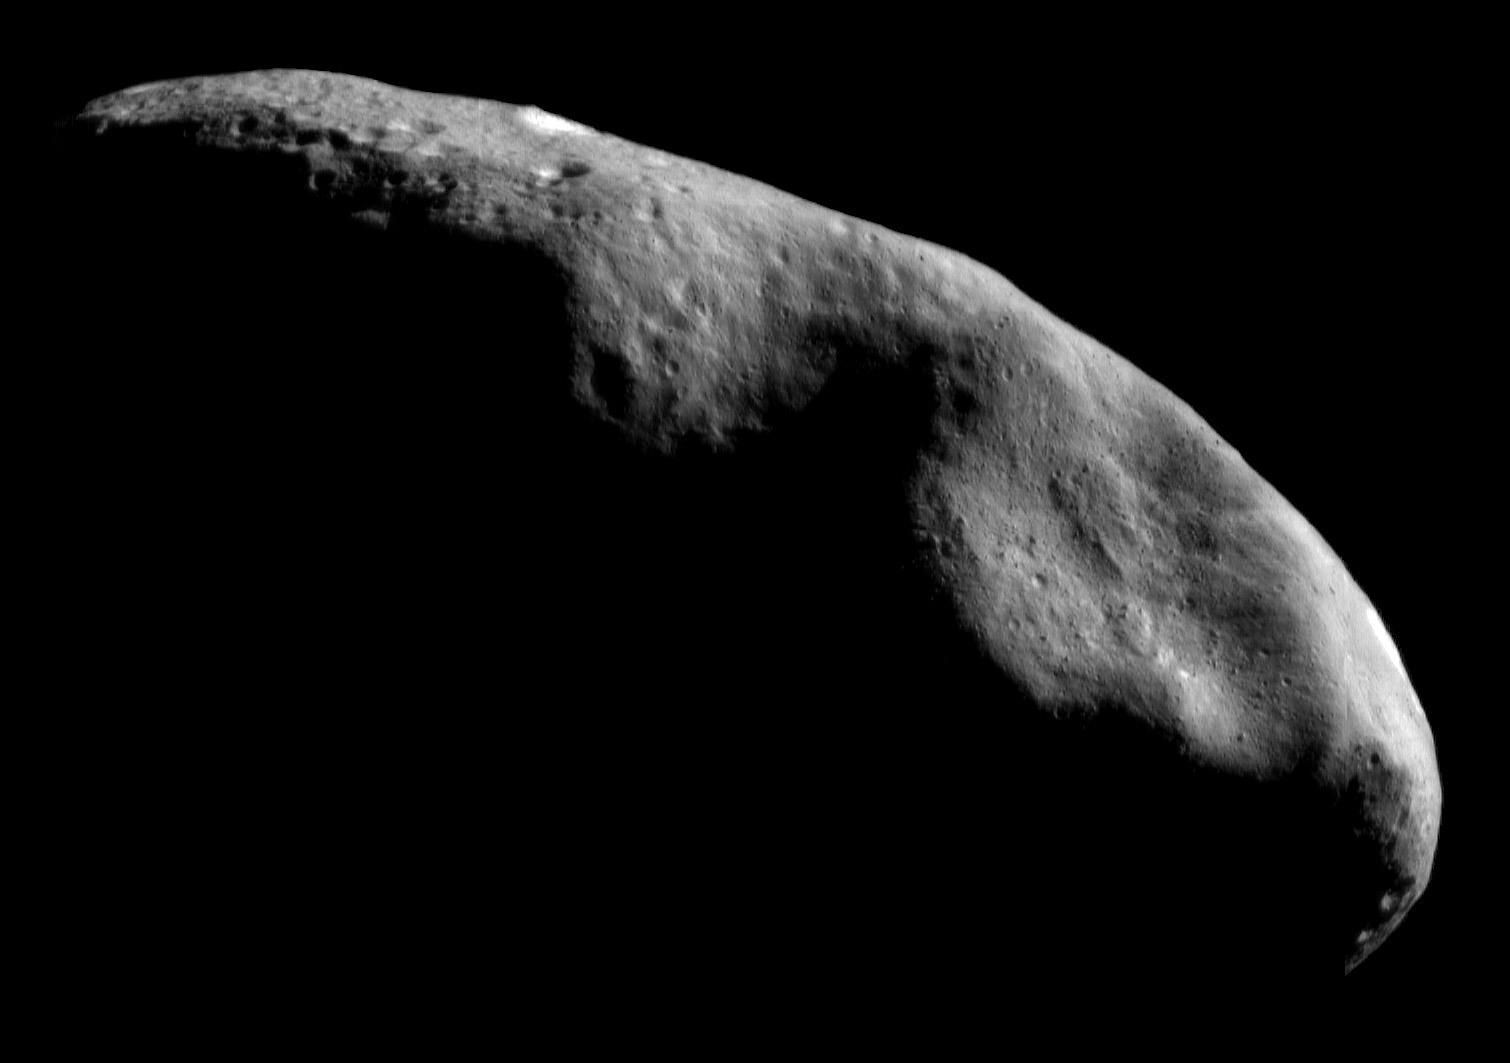
\includegraphics[height=0.35\textheight]{figures/near_mos_20001203_full.jpg}
    \hfill
    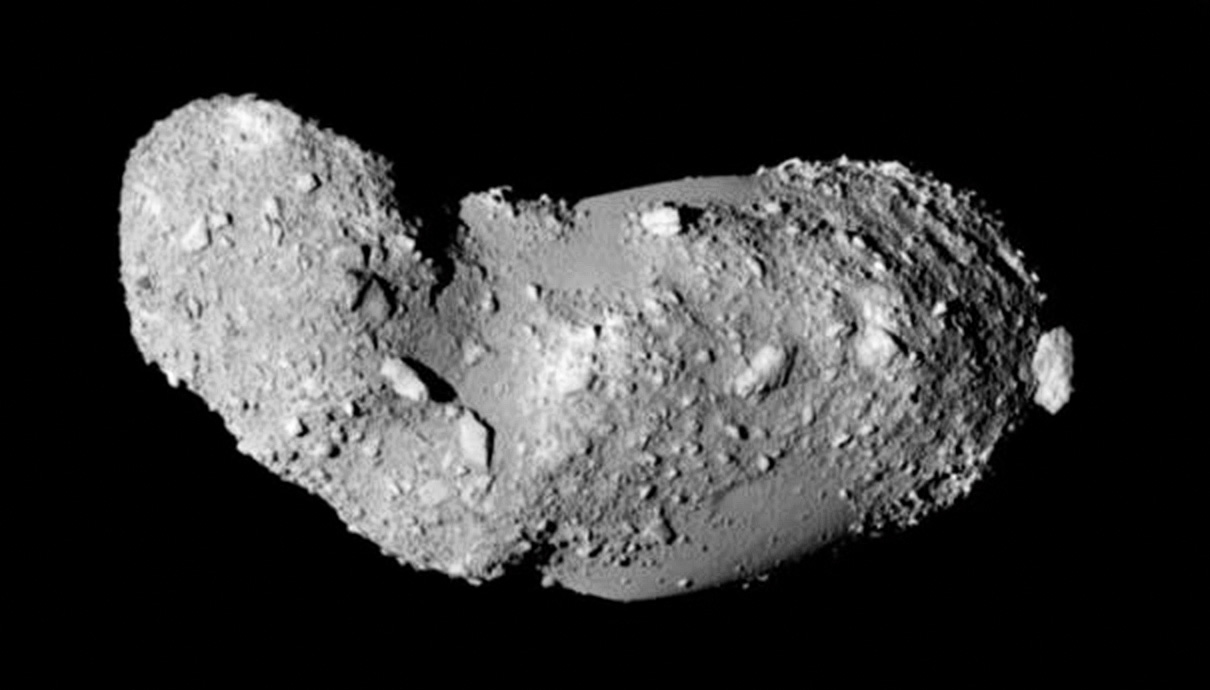
\includegraphics[height=0.35\textheight]{figures/Itokawa8_hayabusa_1210.jpg}
\end{center}
\end{frame}

\begin{frame}{Asteroid Mining}
    \begin{itemize}
      \item Useful materials can be extracted from asteroids to support:
      \begin{itemize}
          \item Propulsion, construction, life support, agriculture, and precious/strategic metals
      \end{itemize}
      \item Commercialization of near-Earth asteroids is feasible~\footfullcite{ross2001}
    \end{itemize}

\begin{center}
\small
    \begin{tabular}{|l|r|r|}
        \hline 
        Element & Price (\SI{}{\$\per\kilo\gram}) & Sales (\SI{}{\$M\per\year}) \\
        \hline \hline 
        Phosphorous (P) & \num{0.08}  & \num{2167} \\
        Gallium (Ga) & \num{300.00}  & \num{1544} \\
        Germanium (Ge) & \num{745.00} & \num{6145} \\
        \hline \hline 
        Platinum (Pt) & \num{12394.00} & \num{1705} \\
        Gold (Au) & \num{12346.00} & \num{49} \\
        Osmium (Os) & \num{12860.00} & \num{307} \\
        \hline
    \end{tabular}
\end{center}

\end{frame}


\begin{frame} %-----------------------------%
\frametitle{Low-thrust vehicles} % electric propulsion
\begin{itemize}
    \item Low-thrust orbital transfers
    \begin{itemize}
        \item Electric propulsion has increased in popularity
        \item Offers much higher specific impulse than chemical engines 
        \item Requires much longer operating periods for maneuvers 
        \item Small satellites with electric propulsion allows for new mission types
            \begin{itemize}
                \item Formation flight (distributed aperture sensing)
                \item On-orbit servicing
                \item Interplanetary swarms
            \end{itemize}
    \end{itemize}
\end{itemize}

\begin{center}
    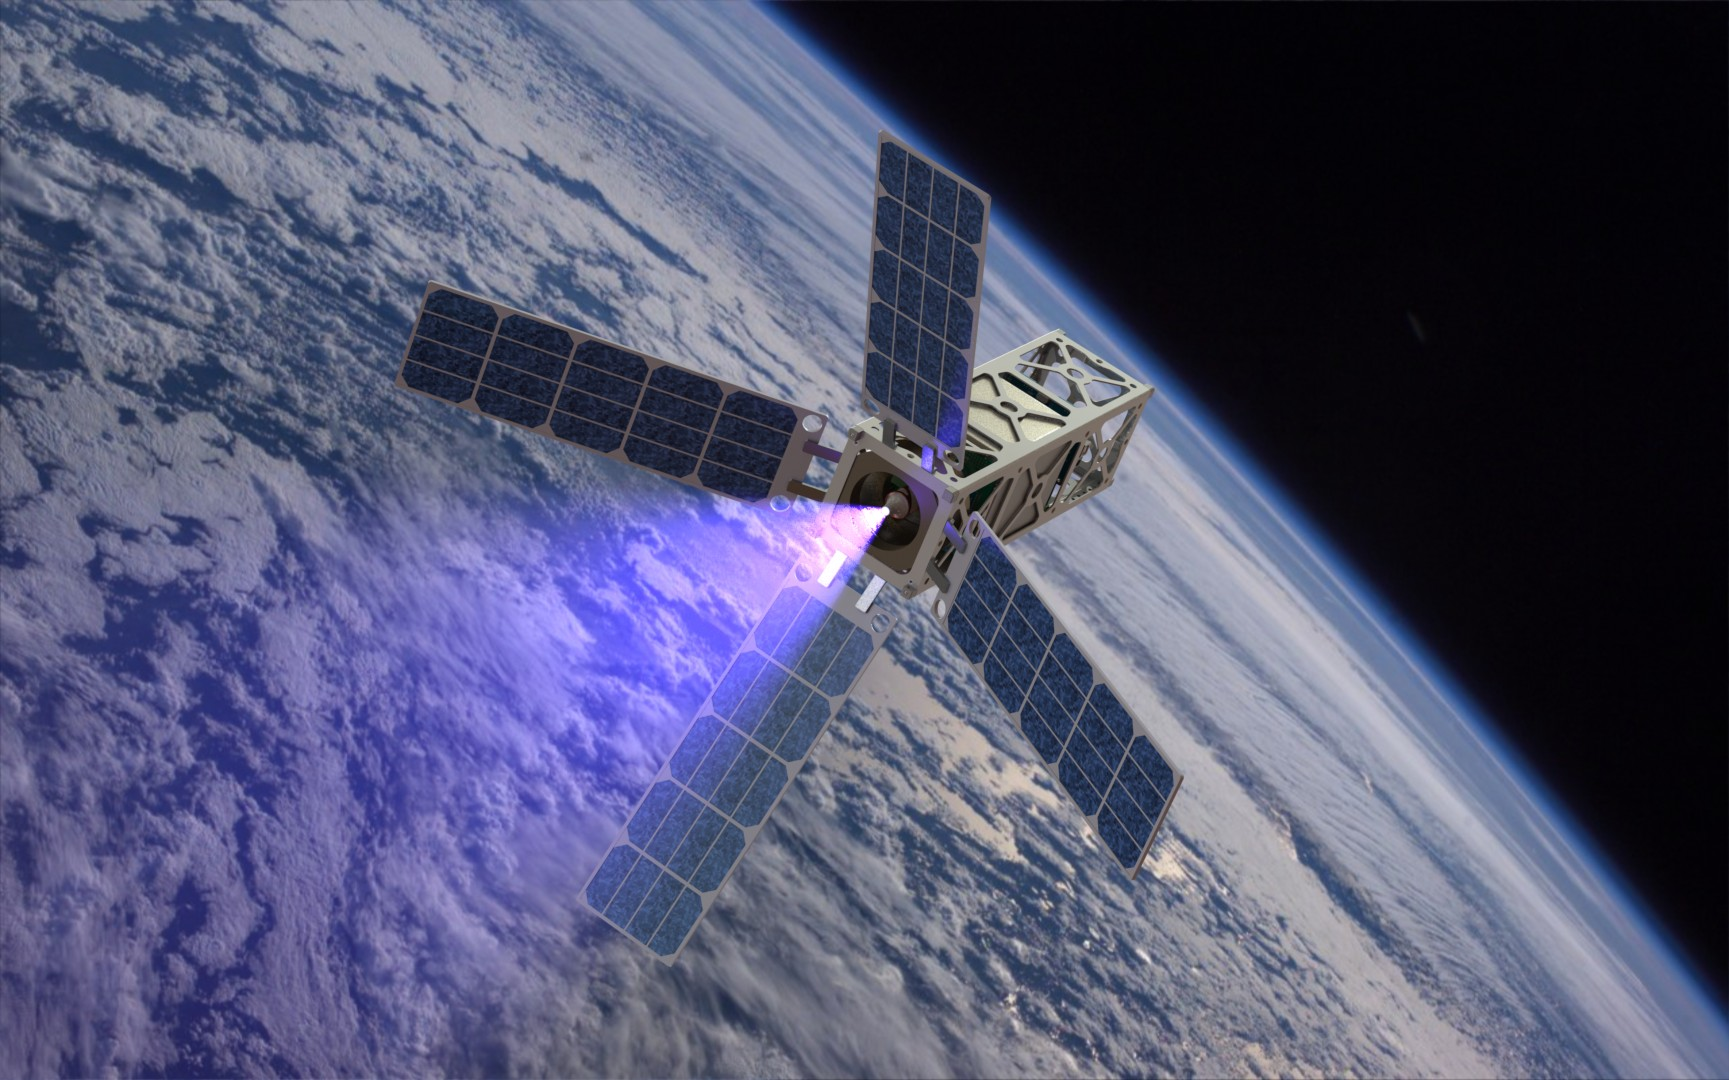
\includegraphics[height=0.3\textheight]{patriot_plume}
    \hfill
    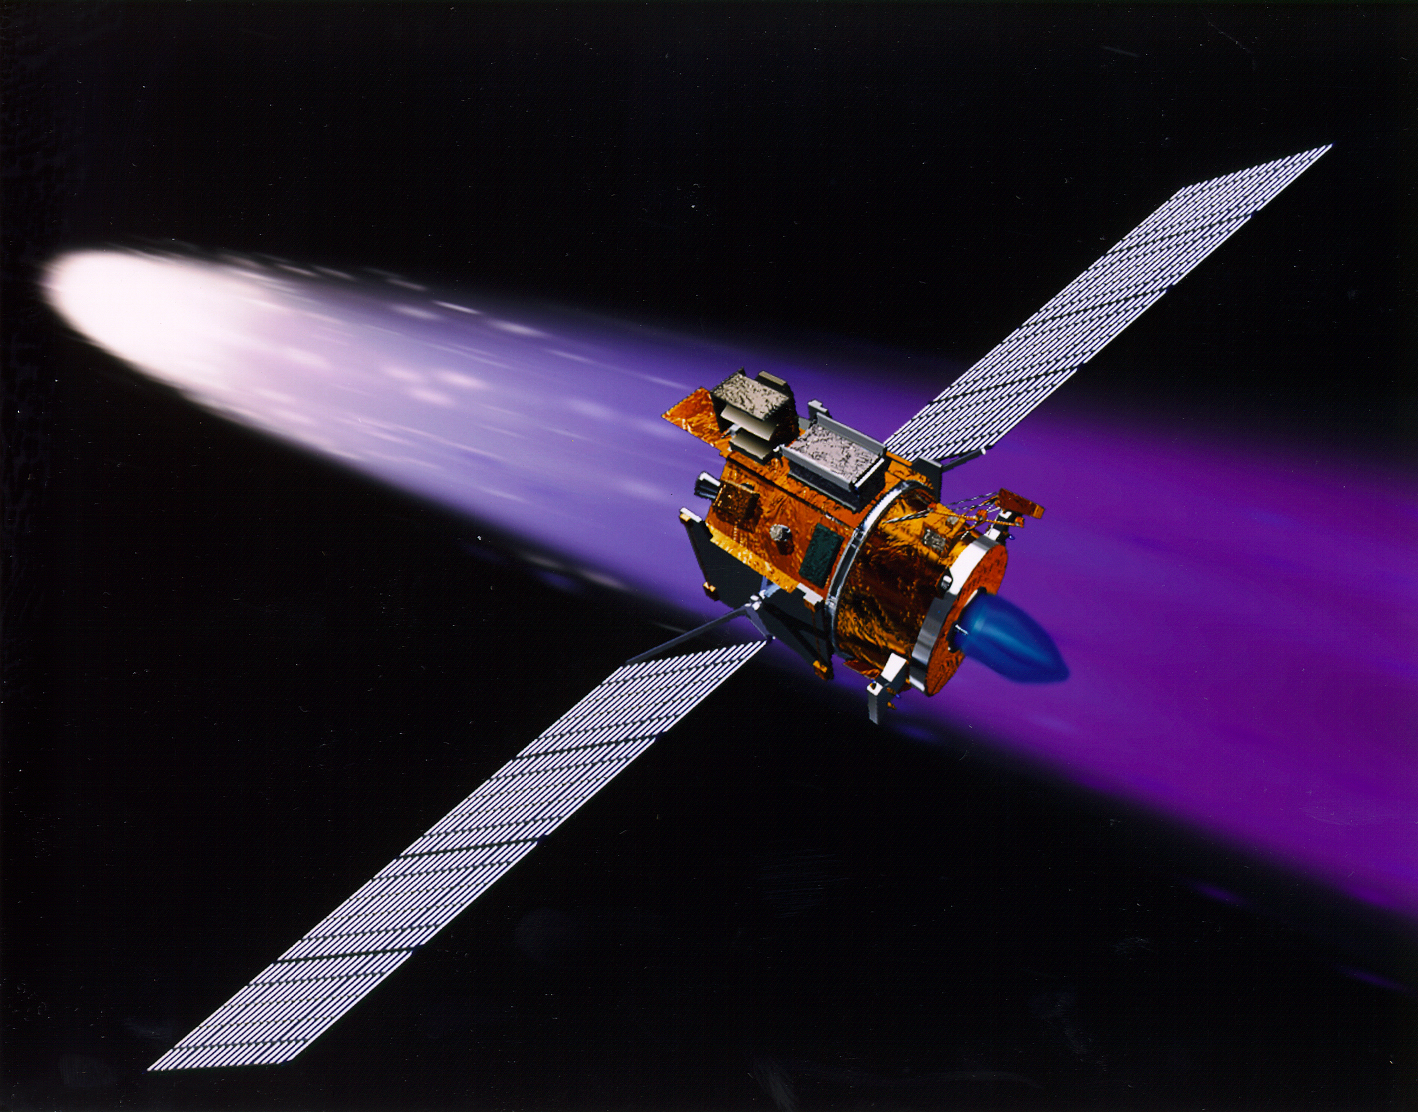
\includegraphics[height=0.3\textheight]{deepspace1}
\end{center}
\end{frame}   %-----------------------------%

\section*{Previous Work}
\subsection*{Past Challenges}

\begin{frame}{Gravitational Modeling} %-----------------------------%
Use a spherical harmonic model to represent gravity field

Much analysis into the structure of dynamics

Hovering type control
\end{frame}   %-----------------------------%

\begin{frame}{Optimal Transfers}
Typically use direct methods

Result in suboptimal solutions

Very difficult to choose correct initial conditions that will achieve convergence
\end{frame}

\section*{Research Approach}
\subsection*{System Model}

\begin{frame}{Polyhedron Gravitation Model}

\begin{itemize}
    \item Globally valid at all points outside of asteroid
    \item Closed-form expression of potential based on asteroid shape 
    \item Exact potential consistent with the resolution of the shape discretization
\end{itemize}
{\small
\begin{align*}\label{eq:potential}
    U(\vecbf{r}) &= \frac{1}{2} G \sigma \sum_{e \in \text{edges}} \vecbf{r}_e \cdot \vecbf{E}_e \cdot \vecbf{r}_e \cdot L_e - \frac{1}{2}G \sigma \sum_{f \in \text{faces}} \vecbf{r}_f \cdot \vecbf{F}_f \cdot \vecbf{r}_f \cdot \omega_f \in \R^1,
\end{align*}
}
Shape based model (show animation of Castalia rotating)
\end{frame}

\begin{frame}{Equations of Motion}
Two body equations of motion

Similarity to the three body problem
\end{frame}


\subsection*{Proposed Approach}

\begin{frame}{Reachability}
Derivable from Optimal control

Developed for safety constraints

Air traffic control example

Recently extended to spacecraft
\end{frame}

\begin{frame}{Reachability Set} % -----------------------------------%

Description of reachability set

Introduce \Poincare section

Generate reachability set on \Poincare section

Use low thrust to enlarge reachability set
\end{frame} %--------------------------------------%

\begin{frame}{\Poincare section}
What is the \Poincare section

Used for determining periodic orbits

Show some plots of periodic orbits
\end{frame}

\begin{frame}{Optimal Control Problem}
Show equations for problem

show constraints

Acceleration limited
\end{frame}

\begin{frame}{Terminal Constraints}
Constraint for section

Constraints for direction

Constraint for control
\end{frame}

\section*{Transfer Example}
\subsection*{Numerical Simulation}

\begin{frame}{Simulation} %-----------------------------%

Describe transfer example

Show animation in both body and inertial frame

Show reachability set

% \animategraphics[autoplay,loop,width=0.5\textwidth]{8}{./animation/single_noavoid/single_noavoid-}{0}{99}~
% \animategraphics[autoplay,loop,width=0.5\textwidth]{8}{./animation/single_avoid/single_avoid-}{0}{99}

\end{frame}%-----------------------------%


\section*{}
\subsection*{}

\begin{frame}{Conclusions} %-----------------------------%

	

\end{frame}   %-----------------------------%

\begin{frame}[c]{Thank you}
	\centering
	
	\textbf{\large Flight Dynamics \& Control Lab} \\
	Mechanical \& Aerospace Engineering \\
	School of Engineering \& Applied Science
	
	\begin{figure} %figure%
       	
\includegraphics[width=0.75\textwidth]{gw_txh_2cs_pos}
  	\end{figure}
	
	\url{https://fdcl.seas.gwu.edu}
\end{frame}


\end{document}

